\subsection{Self-Sovereign Identity}
The idea of the \acrlong{ssi} was born to solve the problems with the current physical and digital identifications.\\
Some of the physical IDs problems are:
\begin{itemize}
    \item The process of obtaining them is time consuming, bureaucratic and costly. For both the ID Owner and Issuer Organization.
    \item If you lose your ID and need to obtain a new one.
    \item Physical IDs can be defrauded with impersonation and ID theft. The only way to check its authenticity is often by contacting the issuing organization.
    \item They are not private.
\end{itemize}
Also, some problems with the current digital IDs are:
\begin{itemize}
    \item Having to register and sign up with different login credentials to every new online service is uncomfortable for the user.
    \item Tedious on-boardings.
    \item Managing multiple passwords is hard and using the same password is a security risk.
    \item The user has no control over what data is being shared and with whom.
    \item The verification of your credentials is dependent on the availability of the issuer.
    \item Third party login services have a financial incentive to collect and store your data.
    \item The user's personal data is stored on the issuer's servers. Centralized storages of personal data create \textit{"honeypots"}. This data is at risk of breaches, leaks or hacks.
\end{itemize}

\acrfull{ssi} is a digital identification scheme in which the user acquires the responsibility of managing how and in what quantity their personal data is used. To do this, it allows the creation of digital \textit{"identity cards"} that can be general for any service or specific for each case. \\
The main characteristics of \acrlong{ssi} are\cite{ssi-guide}:
\begin{itemize}
    \item It is secure and digital peer-to-peer channel is established between Issuer, owner and Verifier.
    \item When credentials are exchanged not even the \acrlong{ssi} system provider knows what is being exchanged.
    \item Credentials are tamper-proof through the use of cryptography.
    \item They are private and under the owner control. \acrshort{ssi} uses Selective Identity disclosure technology.
    \item The Owner chooses what data they want to "show" and is always in control of the relationship with ID Verifiers.
    \item Credentials can be verified anywhere, at any time.
    \item Personal Data is not stored on centralized servers.
    \item \acrshort{ssi} tries to abolish multiple passwords. You just need to know your wallet password.
\end{itemize}

\subsubsection{How does it work?}
In order to explain how the \acrshort{ssi} works, we have to see some concepts previously.
\paragraph{Actors}
The figure \ref{fig:trust-triangle} explains the different actors\cite{ssi-guide} that take place in the process.
\begin{figure}[h]
    \centering
    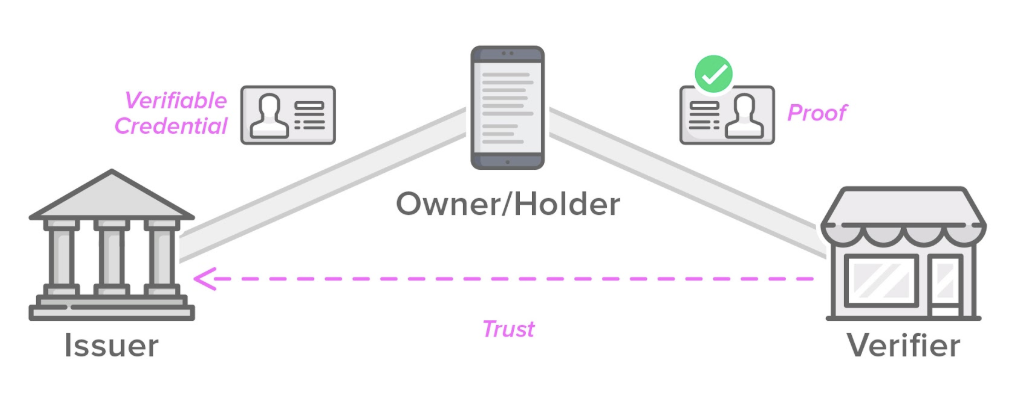
\includegraphics[width=0.7\textwidth]{trust-triangle.png}
    \caption{Trust triangle / Actors in \acrshort{ssi}}
    \label{fig:trust-triangle}
\end{figure}
\begin{itemize}
    \item \textbf{Owner / Holder}: orders the creation of credentials. He stores the credentials locally. He has the power to revoke access to these credentials.
    \item \textbf{Issuer}: provides a digital service. It needs to identify users. Does not need to store user data.
    \item \textbf{Verifier}: creates the credentials with the data provided by the user. It does not store user data (although it has access to it at the time of creation of the credential).
\end{itemize}

\paragraph{Verifiable Credentials}
According to the World Wide Web Consortium \textit{\acrshort{w3c}}\cite{w3c-vc}\footnote{\label{footnote-w3c}More information about Verifiable Credentials and Verifiable Presentations can be found in the main web page of \acrshort{w3c}\cite{w3c-vc}}:
\begin{quote}
    \textit{A verifiable credential can represent all of the same information that a physical credential represents. The addition of technologies, such as digital signatures, makes verifiable credentials more tamper-evident and more trustworthy than their physical counterparts.}
\end{quote}
In the figure \ref{fig:ssi-vc}, we can see clearly the relationship between Issuer, Holder and Verifier and how a Verifiable Data Registry (normally a blockchain) is used to verify the credential's data without the need to contact the issuing party.
\begin{figure}[h]
    \centering
    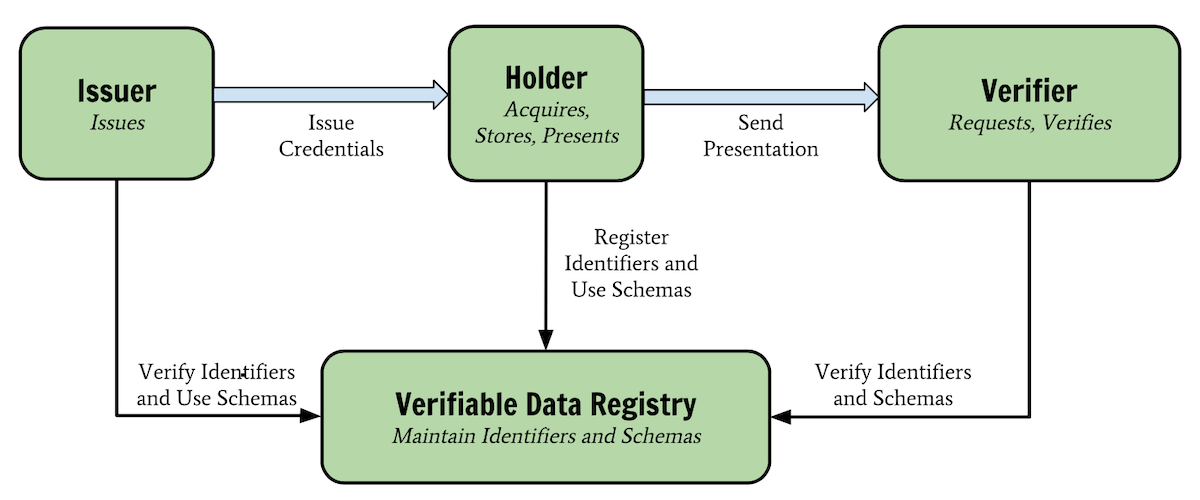
\includegraphics[width=1.0\textwidth]{ssi-vc.png}
    \caption{The roles and information in a \acrshort{ssi} ecosystem by \acrshort{w3c}}
    \label{fig:ssi-vc}
\end{figure}

\paragraph{Verifiable Presentations}
According to \acrshort{w3c}\cite{w3c-vc}\footref{footnote-w3c}:
\begin{quote}
    \textit{A verifiable presentation expresses data from one or more verifiable credentials, and is packaged in such a way that the authorship of the data is verifiable. If verifiable credentials are presented directly, they become verifiable presentations. Data formats derived from verifiable credentials that are cryptographically verifiable, but do not of themselves contain verifiable credentials, might also be verifiable presentations.}

    \textit{The data in a presentation is often about the same subject, but might have been issued by multiple issuers. The aggregation of this information typically expresses an aspect of a person, organization, or entity.}
\end{quote}
In the figure \ref{fig:ssi-vp} we can see the components of a verifiable presentation.
\begin{figure}[ht]
    \centering
    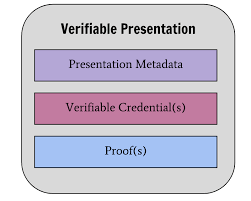
\includegraphics[width=0.5\textwidth]{ssi-vp.png}
    \caption{Basic components of a verifiable presentation by \acrshort{w3c}}
    \label{fig:ssi-vp}
\end{figure}
\paragraph{Decentralized Identifiers (DIDs)}
According to \acrshort{w3c}\cite{w3c-did}\footnote{More information about the \acrshort{did}s can be found in the main web page of \acrshort{w3c}\cite{w3c-did}}:
\begin{quote}
    \textit{\acrfull{did}s are a new type of identifier that enables verifiable, decentralized digital identity. A \acrshort{did} identifies any subject (e.g., a person, organization, thing, data model, abstract entity, etc.) that the controller of the \acrshort{did} decides that it identifies. In contrast to typical, federated identifiers, \acrshort{did}s have been designed so that they may be decoupled from centralized registries, identity providers, and certificate authorities. Specifically, while other parties might be used to help enable the discovery of information related to a \acrshort{did}, the design enables the controller of a \acrshort{did} to prove control over it without requiring permission from any other party. \acrshort{did}s are URIs that associate a \acrshort{did} subject with a \acrshort{did} document allowing trustable interactions associated with that subject.}

    \textit{Each \acrshort{did} document can express cryptographic material, verification methods, or service endpoints, which provide a set of mechanisms enabling a \acrshort{did} controller to prove control of the \acrshort{did}. Service endpoints enable trusted interactions associated with the \acrshort{did} subject. A \acrshort{did} document might contain the \acrshort{did} subject itself, if the \acrshort{did} subject is an information resource such as a data model.}
\end{quote}

\paragraph{Wallets}
A wallet\cite{ssi-wallets} is a private repository that allows its owner to store, manage, and present keys and identity credentials.\\

Some of the properties every wallet should have are:
\begin{itemize}
    \item Provide secure access to the owner.
    \item Guarantee that only authorized entities can access to it.
    \item Ensure security and data encryption.
    \item Provide recovery for keys and credentials.
    \item Be connected to the blockchain where the \acrshort{did} was registered.
    \item Provide mechanism for subjects and issuers to change the status of their credentials.
    \item Provide mechanism for the owner to erase all the data associated with them.
\end{itemize}
Normally, when we talk about wallet, we think in mobile wallets (mobile applications), but a wallet can also be in a desktop, browser, hardware or the cloud.

\paragraph{Functioning}
In the architecture\cite{how-to-ssi} we find a credential provider (\textit{issuer}) that is responsible for signing the data provided by the user by creating a certificate. Then, it will be signed by the user, attesting that the certificate generated by the issuer does not contain missing or altered information.\\

Signatures by both the user and the issuer are performed using DIDs, which are traditional asymmetric keys. The public key of both is stored publicly on the blockchain. In this way, later on, the service provider (\textit{verifier}) that wants to identify the user will only have to verify that the signatures are correct and that, therefore, the credential has not been altered and contains the same information that the user provided to the identity provider.\\

In the next figure (figure \ref{fig:ssi-scheme}) we can see a graphic scheme of the explained above.
\begin{figure}[h]
    \centering
    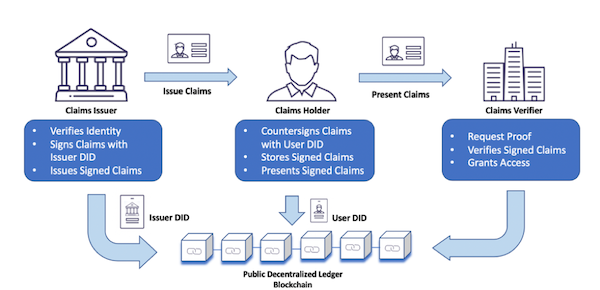
\includegraphics[width=1.0\textwidth]{how-to-ssi.png}
    \caption{SSI functioning scheme}
    \label{fig:ssi-scheme}
\end{figure}

\subsubsection{Use cases}
\acrlong{ssi} is benefiting several industries\cite{ssi-guide}, some examples are: streamlining bureaucratic procedures, improving a more efficient healthcare system, detecting academic and business fraud, creating a better user experience while onboardings or helping companies avoid personal data breaches and \acrshort{gdpr}\cite{gdpr} fines.

\subsubsection{Alastria}
Alastria (figure \ref{fig:alastria_logo}) is the world's first nation-wide, multi-sectorial, enterprise grade, permissioned blockchain network. A non-profit association open to all types of companies and organizations with the mission to contribute to the creation of a diverse innovation ecosystem. Alastria is technology agnostic and offers the networks promoted by its partners as well as a user centric Digital Identity model, the Alastria ID, focused on ensuring the legal validity of the transactions on the networks.
\begin{figure}[h]
    \centering
    
\includegraphics[width=0.5\textwidth]{alastria-logo.png}
    \caption{Alastria logo}
    \label{fig:alastria_logo}
\end{figure}
\paragraph{Alastria ID}
Alastria ID (figure \ref{fig:alastria_id_logo}) is a digital identity model proposed by the Consortium for use in digital services, even beyond blockchain technology itself and inspired by the Self Sovereign Identity concept.\\
\begin{figure}[h]
    \centering
    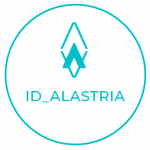
\includegraphics[width=0.2\textwidth]{alastria-id-logo.png}
    \caption{Alastria ID logo}
    \label{fig:alastria_id_logo}
\end{figure}

The Identity Commission of Alastria ID\cite{alastria-context} has taken a further step in the typical functionalities of this tool. It has followed the recommendations of the ID of the \acrfull{w3c}\cite{w3c}, the international community that develops Internet standards. It has even been improved. Alastria ID has been developed in accordance with the demanding \acrfull{gdpr}\cite{gdpr} (General Data Protection Regulation), and \acrfull{eidas}\cite{eidas}..\\

The Alastria Standards Commission, which participates in all international and national standardization bodies, has collaborated in the process of the definition of the Alastria ID. The model specification inspired the Spanish identity standard UNE 71307\cite{une-71307} and the decentralized identity framework of EBSI\cite{ebsi} (European Blockchain Services Infrastructure), the blockchain of European public administrations.\\

In the next section we will delve into the peculiarities and details of the different tools created by Alastria to facilitate the use of Alastria ID.

\subsubsection{Other implementations}
At present, \acrlong{ssi} is still at an early stage. However, there is already an extensive catalog of projects that show their potential. Different working groups and standardization agencies have been working to develop new standards and protocols that are the base of the \acrshort{ssi} model\cite{ssi-wallets}. Some of these groups are: the \textit{\acrfull{dif}}, the \textit{\acrfull{ebsi}}, the \textit{\acrfull{ietf}}, \textit{LACChain}, \textit{NIST}, \textit{Sovrin}, \textit{OASIS}, the \textit{\acrfull{oidf}}, and the \textit{\acrfull{w3c}}.\\

There are also a few existing solutions on the market which leverage new standards and protocols for \acrshort{ssi}:
\paragraph{Serto/uPort}
Serto\cite{serto} (figure \ref{fig:uport}) formerly known as uPort\cite{uport} is a web-based wallet and identity management system created by ConsenSys\cite{consenSys}. This project allows users (people) to manage their own private and public keys, without the need for intermediaries. It allows these keys to be recovered without the user having to lose their identity. The system consists of a mobile application (wallet), where the user can manage their identity, can receive and issue claims. A claim is nothing more than a data structure where \textit{"someone says something about another person"}. These claims make up the identity of the user, and can be displayed to identify themselves in front of entities. The identity is controlled by the user, without problems of someone questioning the legitimacy or altering the identity data.
\begin{figure}[h]
    \centering
    
\includegraphics[width=.2\textwidth]{serto-logo.png}\hfill
    
\includegraphics[width=.2\textwidth]{uport-logo.png}\hfill
    
\includegraphics[width=.3\textwidth]{consensys-horizontal-logo.png}
    \caption{Serto, uPort and ConsenSys logos}
    \label{fig:uport}
\end{figure}

\paragraph{David19}
David19\cite{david19} (figure \ref{fig:david19}) emerges as a collaborative application in which any citizen can participate to promote digital transformation in order to face health emergencies caused by the COVID-19 pandemic in 2019. This project created by LACChain\cite{lacchain} allows users (citizens) to share their information in solidarity, in a secure and anonymous way through self-claimed credentials. With this information, risk maps can be generated in real time, thus allowing authorities to make key decisions in managing the pandemic.\\
\begin{figure}[h]
    \centering
    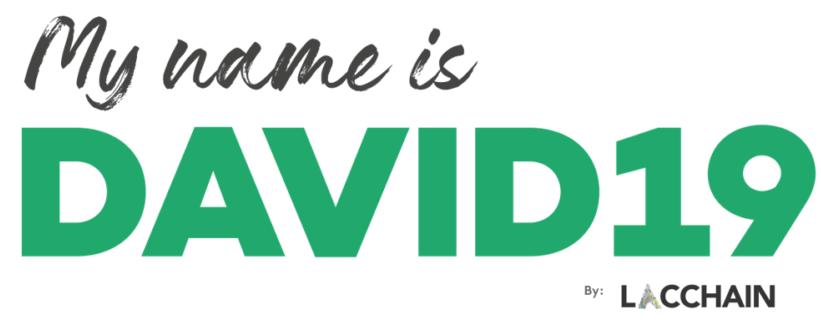
\includegraphics[width=.3\textwidth]{logo-david19.png}
    \caption{David19 logo}
    \label{fig:david19}
\end{figure}

In a second phase\cite{que-es-david19}, it is proposed that the entities join the ecosystem, and that they can issue more sophisticated credentials, such as permits to return to work, medical certifications or academic degrees. The ultimate goal of David19 is for a person to only need a mobile device (wallet) to demonstrate that they are fit to get on a plane, return to work, visit a museum, etc., all in compliance with applicable regulations. The final objective of David19 is that a person only needs a mobile device (wallet) to demonstrate that they are healthy to get on a plane, return to work, visit a museum, etc., all in compliance with the regulations that apply at the time and the place.

\paragraph{Hyperledger Indy}
Contributed by the Sovrin Foundation\cite{sovrin-yt,sovrin}, Hyperledger Indy\cite{indy-gh,indy} (figure \ref{fig:indy}) enables people to manage and control their digital identities. Rather than companies storing large amounts of personal data, what they store are indicators of identity. One of Hyperledger Indy's key tenets is its privacy-by-design approach: \textit{"it's not about protecting data but about designing so, that data doesn't need protection"}.\\
\begin{figure}[h]
    \centering
    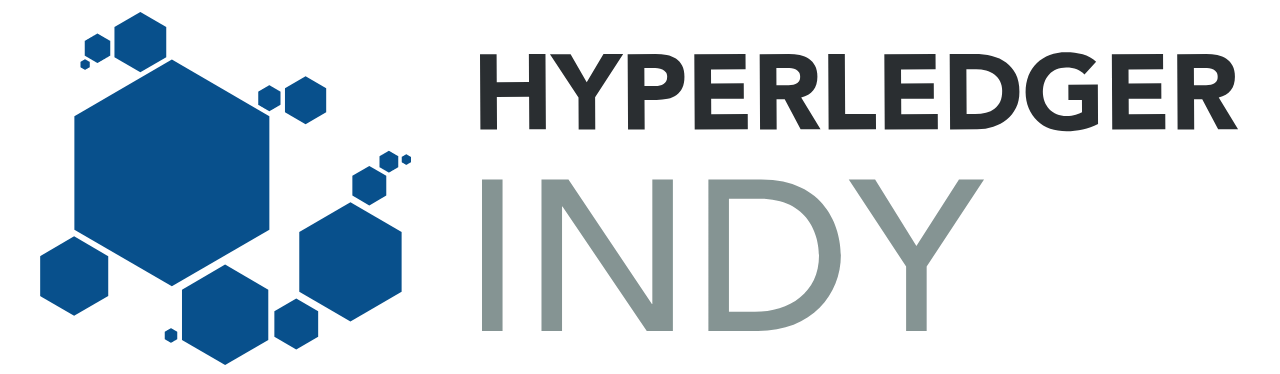
\includegraphics[width=.3\textwidth]{hyper-indy.png}
    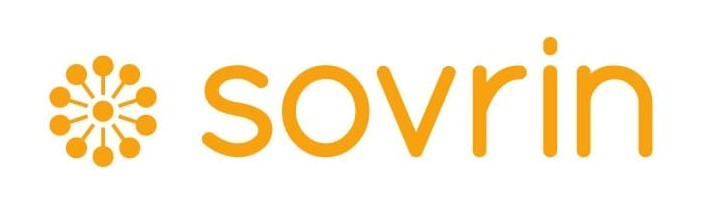
\includegraphics[width=.3\textwidth]{Sovrin-Logo.jpg}\hfill
    \caption{Hyperledger Indy and Sovrin logos}
    \label{fig:indy}
\end{figure}

The proposal is based on having multiple \acrshort{did}s for each user. Every time an agent is operated to give the user's credentials, a new \acrshort{did} will be generated.\\

There are also other solutions\cite{ssi-wallets} like \textit{Evernym}, \textit{KayTrust} (by Everis) and \textit{Rem} (by World Data).
